%% Dieser Quelltext ist in der Kodierung UTF-8 zu speichern und mit lualatex
%% zu kompilieren.

% !TeX program = lualatex

\documentclass{scrartcl}  % KOMA-Scritp equivalent to \documentclass{article}
% \documentclass[12pt,a4paper]{article}
% \usepackage[utf8]{inputenc}
% TODO: fix \setdefaultlanguage problem while compiling
% \setdefaultlanguage[spelling=new, babelshorthands=true]{german}  
\usepackage{polyglossia}  % for LuaLatex
\usepackage{fontspec}  % for LuaLatex
\usepackage{luacode}  % for LuaLatex
\renewcommand{\familydefault}{\sfdefault}  % change serif (default-value) to SansSerif version of LaTex-font
\usepackage{amsmath}  % recommended as an adjunct to serious mathematical typesetting
\usepackage{amsfonts}  % extended set of fonts for use in mathematics
\usepackage{amssymb}  % allows the use of various special characters and symbols
\usepackage{graphicx}  % providing interface for optional arguments to the \includegraphics command
\usepackage{array}  % extended implementation of the array and tabular environments
\usepackage[table]{xcolor}  % for coloring rows in tables, load before \usepackage{xcolor}!!!
\usepackage{xcolor}  % to use broader color plate
\usepackage{hyperref} % to create hypertext links in PDF (jump from content overview to according pages)
\usepackage{enumitem} % for enumerate with letters
\usepackage{textcomp} % for copyright symbol
\usepackage{tcolorbox} % for making boxes around stuff
\usepackage{wrapfig}  % to wrap images and text
\usepackage{lipsum}  % generates filler text
\usepackage{pdflscape}  % for using landscape format in between
\usepackage{smartdiagram}  % to create cooler diagrams
\usepackage{floatrow}  % provides many ways to customize layouts of floating environments
\usepackage{caption}  % for more formating options for captions
\usepackage{gensymb}  % to use symbols
\usepackage{siunitx}  % to use symbols and units
\usepackage[scale=1.5]{ccicons}  % for Creative Commons icons
\usepackage{tikz}  % use for spiderweb diagram
\usepackage{pdfpages}  % include external PDFs

% needed for chemistry notations
\usepackage{chemmacros}  % used for chemistry stuff
\usepackage{chemfig}  % used for chemistry stuff
\usepackage[version=4]{mhchem}   % used for chemistry stuff
\usepackage{modiagram}  % to draw AO (atom orbitals) and MO diagrams
\usepackage{bohr}  % to draw BOHR modells of atoms (till Element 112)
\usepackage{elements}  % collection of data of elements (till Element 112)

% TODO: pst-labo works in pdflatex but not lualatex...work out, wthat and how to fix
% pstricks  
%\usepackage{auto-pst-pdf}
%\usepackage{pst-labo}


% libraries
\tcbuselibrary{skins}  % for textcolorbox
\usetikzlibrary{shapes}


% page layout for worksheets
\usepackage[left=1.50cm, right=1.50cm, top=2.00cm, bottom=2.00cm]{geometry}
\usepackage[headsepline,footsepline]{scrlayer-scrpage}
%scrpage2
\pagestyle{scrheadings}
\setlength{\parindent}{0pt}  % no indentation of paragraphs

% this luacode has no function, except to make sure the document is compiled using LuaLaTex
\begin{luacode*}
	--[[
		print("this is just a comment")
	--]]
\end{luacode*}


% Information for Header and Footer
% *********************************

\ihead{Chemie}
\chead{\textbf{Zombie School}}
\ohead{2021}
% \ohead{90min}
% \ifoot{Fußzeile innen}
\cfoot{\textsf{\pagemark}}
%\ofoot{Fußzeile außen}


\author{Jonas Pews}
\title{Zombie School - Mission 2: Die Struktur der Kohlenwasserstoffe}
\date{\today}

% Some Info about this document
% *****************************
%
% TODO: write Text how this doc can be used in school. also about RLP Brandenburg/Berlin

% TODO: write more comments to explain/comment :-) the Tex-Code 

% Info for tabing in tex file
% ***************************
% part/section is one tab
% subsection is two tab
% pagebreak/layout changes (landscape) always no tab

\begin{document}

	\begin{center}
		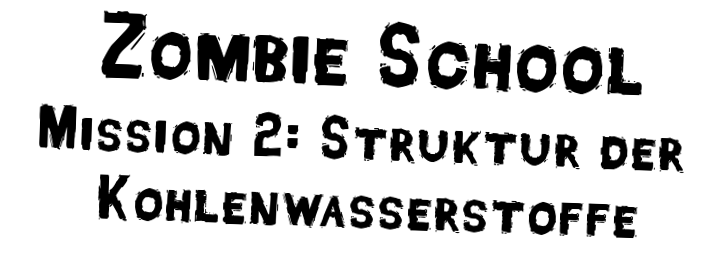
\includegraphics{img/headline_ch_02_chStrukturKW}
	\end{center}	
	
	\begin{center}
		{\LARGE \textbf{Mach dich mit den Chemikalien vertraut!}}
	\end{center}
	
\vspace{0.7cm}	
	\textit{Na super, draußen Zombies, drinnen kein Netflix und nur Schulbücher! Du überlegst kurz, die Flucht nach vorne anzutreten, aber der Schokoriegel im sicheren Schulgebäude überzeugt dich hierzubleiben und den Tipps deiner Lehrkraft zu folgen.} \newline

\vspace{0.7cm}	

	\textbf{Ziel: Finde heraus, woraus Kohlenwasserstoffe bestehen.}
	\begin{enumerate}
		\item Führe die Experimente durch und protokolliere sie in deinen Unterlagen.
		\item Löse alle Arbeitsuafträge für die Auswertung. 
		\item Erkläre deiner Lehrkraft am Ende, wie die Kohlenwasserstoffe aufgebaut sind.
	\end{enumerate}

\vspace{0.7cm}	
	\begin{minipage}{0.7\textwidth}
		\noindent \textbf{Am Ende dieses Kapitels sollst du ... :}
		\begin{enumerate}
			\item ... beschreiben können, dass Kohlenwasserstoffe Verbindungen sind, die aus Kohlenstoffatomen und Wasserstoffatomen aufgebaut sind.
			\item ... den Unterschied zwischen Strukturformel (\textit{LEWIS-Formel}) und Summenformel erklären können.
		\end{enumerate}
		\textbf{Vorgehensweise:}
		\begin{enumerate}
			\item Arbeite in Gruppen von 4-5 SuS um das Experiment durchzuführen.
			\item Bearbeite die Arbeitsaufträge allein.
		\end{enumerate}
			
	\end{minipage}
	\hspace{0.1\textwidth}
	\begin{minipage}{0.2\textwidth}
		\begin{tcolorbox}
			[enhanced,
			width=0.9\textwidth,
			colback=white,
			colframe=black,
			fonttitle=\sffamily\bfseries\large, 
			title=Zeit,  % search keyword::Zeit
			attach boxed title to top center={xshift=-0.0mm,yshift=-0.50mm},
			boxed title style={skin=enhancedfirst jigsaw,size=small,arc=1mm,bottom=-1mm,colframe=black,height=0.75cm},
			colbacktitle=black,
			drop lifted shadow]
			\centering
			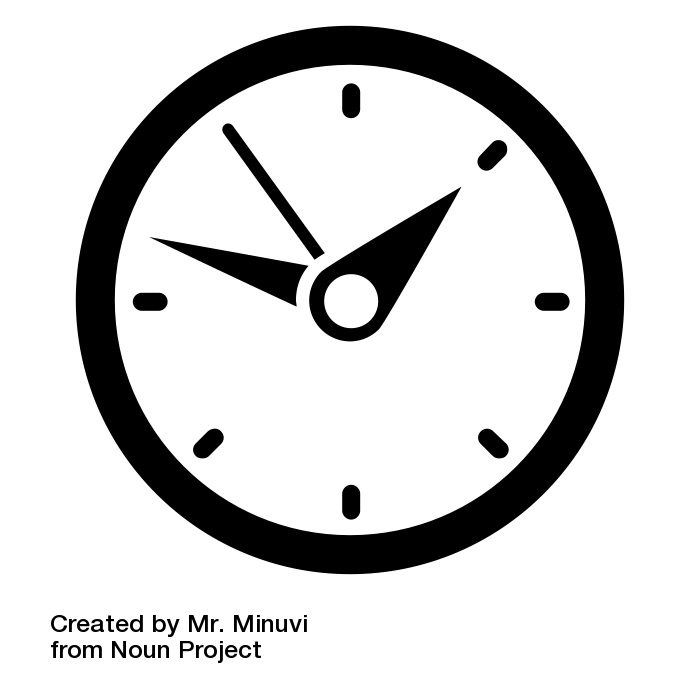
\includegraphics[width=0.9\textwidth]{../symbols/symbol_tex_time}
			
			\begin{center}
				\textbf{90min}
			\end{center}
		\end{tcolorbox}
	\end{minipage}

\newpage	
	\section{Experiementelle Untersuchung von Kerzenwachs}
			
		\noindent \textbf{Auftrag: Untersuche experimentell die Zusammensetzung einfacher organischer Verbindungen und leite daraus die Struktur von Methan her!}
		
		\begin{enumerate}
			\item Führe das \textbf{Experiment} durch und \textbf{protokolliere} es.
			\item Beantworte die gegebenen Fragen (siehe unten) in deiner Auswertung.
		\end{enumerate}
		
		\begin{tcolorbox}[enhanced,
			colback=white,
			colframe=green!30!black,
			fonttitle=\sffamily\bfseries\large, 
			title=Durchführung,
			attach boxed title to top left={xshift=3.2mm,yshift=-0.50mm},
			boxed title style={skin=enhancedfirst jigsaw,size=small,arc=1mm,bottom=-1mm,colframe=green!50!black,height=0.75cm},
			colbacktitle=green!50!black,
			% shadow={2mm}{-1mm}{0mm}{black!20!white}
			drop lifted shadow]
			\begin{wrapfigure}{L}{0.15\textwidth}  
				\centering
				\vspace{-14pt}  % to align image with first line of text
				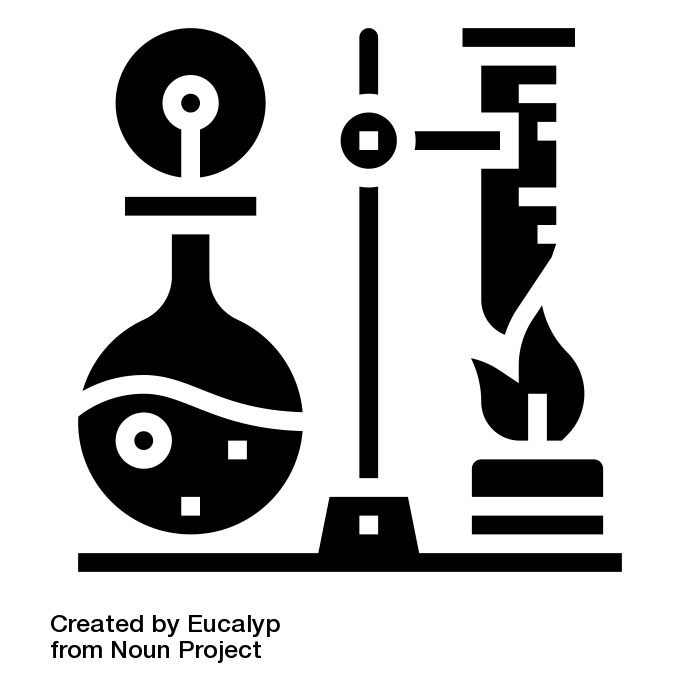
\includegraphics[width=0.9\textwidth]{../symbols/symbol_tex_method}
			\end{wrapfigure}
			
			Halte ein brennende Kerze unter die Öffnung eines kleinen Becherglases oder Reagenzglases. Prüfe die kondensierte Flüssigkeiten mit weißem Kupfersulfat\footnote{Falls deine Lehrkraft Watesmo-Papier hat, kannst du auch das nutzen.}. \newline 
			Wasche ein Reagenzglas mit einigen Tropfen Bariumhydroxid-Lösung aus. Halte die brennende Kerze wieder unter die Öffnung des Reagenzglases\footnote{Falls es kein Feuerzeug gibt, frag deine Lehrkraft nach einer Kerze.}.
			\vspace{0.7cm}  % to fill empty space in tcolorbox
		\end{tcolorbox}
	
		\vspace{0.5cm}
		
		\noindent \textbf{Fragen für die Auswertung}
		
		\begin{enumerate}
			\item Leite aus deinen Beobachtungen her, aus welchen Elementen Methan besteht. Der Brennstoff in der Kerze ist chemisch sehr ähnlich und besteht aus den gleichen Elementen.
				\begin{itemize}
					\item \textbf{Nenne} die Gase, die bei der Verbrennung entstehen. Du hast sie gerade nachgewiesen.
					\item \textbf{Nenne} die beiden Elemente, die sich bei der Verbrennung mit Sauerstoff  verbinden, um diese Gase zu bilden? (\textbf{Hinweis:} Besprich deine Ergebnisse mit der Lehrkraft, falls du dir nicht sicher bist.)
				\end{itemize}
			\item Leite aus deinen Erkenntnissen die Struktur von Methan mit Hilfe der gegebenen Fragen her.
				\begin{itemize}
					\item \textbf{Zeichne} das BOHR'sche Atommodell für beide Elemente.
					\item \textbf{Zeichne} anschließend die LEWIS-Formel für beide Elemente.
					\item \textbf{Erläutere} wie sich beide Elemente verbinden müssen, damit sie beide die Oktettregel erfüllen (\textbf{Hinweis:} Besprich deine Ergebnisse mit der Lehrkraft, falls du dir nicht sicher bist.).
				\end{itemize}
			\item Stelle die ausgeglichene Reaktionsgleichung für die Verbrennung von Methan auf.
		\end{enumerate}
	
		\begin{tcolorbox}[enhanced,
			colback=white,
			colframe=black,
			fonttitle=\sffamily\bfseries\large, 
			title=LEWIS-Strukturformeln,  % search keyword::URL
			attach boxed title to top left={xshift=3.2mm,yshift=-0.50mm},
			boxed title style={skin=enhancedfirst jigsaw,size=small,arc=1mm,bottom=-1mm,colframe=black,height=0.75cm},
			colbacktitle=black,
			drop lifted shadow]
			\begin{wrapfigure}{L}{0.15\textwidth}  
				\centering
				\vspace{-14pt}  % to align image with first line of text
				
\includegraphics[width=0.9\textwidth]{img/musstewissen_lewis}
			\end{wrapfigure}
			
			\textbf{LEWIS-Strukturformeln} sehen schwerer aus, als sie es sind. Hier kannst du dich noch einmal darüber informieren, wie man diese Strukturen zeichnet und was sie genau bedeuten\footnote{Wenn du den QR-Code nicht scannen kannst, kannst du auch direkt aus der PDF-Datei auf die URL klicken}. \newline
			\textbf{Quelle} [Stand:12.2.2020]: \newline 
			\url{https://www.youtube.com/watch?v=toQD3nPZQn4}
			\vspace{0.5cm}  % to fill empty space in tcolorbox
		\end{tcolorbox}	

	

\end{document}

